%+----------------------------------------------------------------------------+
%| SLIDES: main file
%| Contents:	- 60 minutes (extimated duration 3 minutes per slide )
%|				- 10 slides  Introduction and Background
%|				- 10 slides  Results
%| Author: Antonio miti
%| Place: 
%| Date: 
%+----------------------------------------------------------------------------+


%- HandOut Flag -----------------------------------------------------------------------------------------
	\newif\ifHandout
	\Handouttrue  %uncomment for the printable version
	%Handling of flags it is not preserved when passing to standalone-subfiles!


%- D0cum3nt ----------------------------------------------------------------------------------------------
\ifHandout
	\documentclass[handout,10pt]{beamer}   
	\setbeameroption{show notes} %print notes   
\else
	\documentclass[10pt]{beamer}
\fi




%- Packages ----------------------------------------------------------------------------------------------
\usepackage{custom-style}
\usepackage{math}


%--Beamer Style-----------------------------------------------------------------------------------------------
\usetheme{toninus}


\usetikzlibrary{backgrounds}
  \tikzset{
    invisible/.style={opacity=0},
    visible on/.style={alt=#1{}{invisible}},
    alt/.code args={<#1>#2#3}{%
      \alt<#1>{\pgfkeysalso{#2}}{\pgfkeysalso{#3}} % \pgfkeysalso doesn't change the path
    },
  }



%- T1tle P4g3 -------------------------------------------------------------------------------------------
\title{A canonical morphism between \\ twisted and untwisted higher Courant \texorpdfstring{$L_\infty$}{Lie infinity} algebras} 
\subtitle{\href{https://www.mat.uniroma2.it/~kowalzig/ws.html}{Geometry \& Topology in Rome}}
\author[AMM]{\href{www.antoniomiti.it}{Antonio Michele Miti}}
%\institute[UCSC and KU Leuven]{
%  \begin{tabular}[h]{ccc}
%      Università Cattolica del Sacro Cuore & $\qquad$ & KU Leuven \\
%      Brescia, Italy & & Leuven, Belgium \\
%      \href{https://dipartimenti.unicatt.it/dmf-home?rdeLocaleAttr=it}{
\includegraphics[width=3.5cm]{Logos/UnicattBS-logo}} & & 
%      \href{https://wis.kuleuven.be/english}{
\includegraphics[width=4cm]{Logos/KULeuven_logo}}
%  \end{tabular}      
%}
%\institute[Mpim]{
%	MPIM, Bonn, Germany 
%	\\
%	\vspace{.5em}
%	\href{https://www.mpim-bonn.mpg.de/}{
\includegraphics[width=6cm]{./Logos/Mpim_logo}}
%}
\institute[SUR]{
	Sapienza Università di Roma \\
	Rome, Italy 	\\
	\vspace{.5em}
  \begin{tabular}[h]{ccc}
      \href{https://dipartimenti.unicatt.it/dmf-home?rdeLocaleAttr=it}{
\includegraphics[width=6cm]{./Logos/Sur_logo}} & & 
      \href{https://wis.kuleuven.be/english}{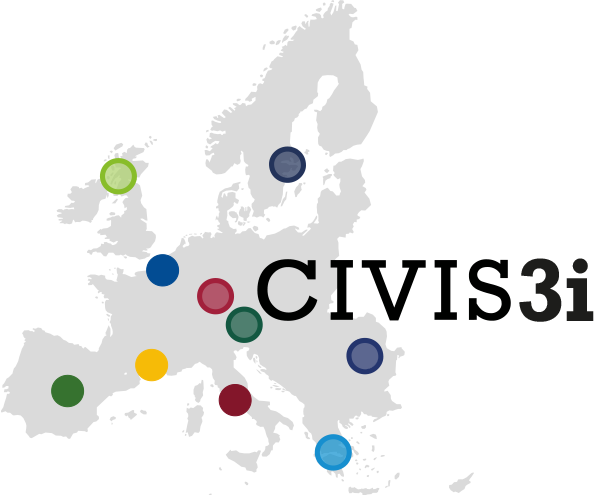
\includegraphics[width=3cm]{Logos/Civis_logo}}
  \end{tabular}    
}
\date[Template_21] % (optional, should be abbreviation of conference name)
{	
	{\vskip 1ex}
	Roma,
	\\
	July 4, 2025
}





\newcommand{\thankyouslide}[0]{
	\ifHandout

	\else
		\addtocounter{framenumber}{-1}
		\begin{frame}{}
		\label{frame:thankyouslide}
			\vfill
		  \centering 
		  {\Huge\color{red} 
		  \emph{Thank you for your attention!}}
			\vfill
			%
			\centering
			\fbox{
				Picture or Take-away message.
				% 		\includegraphics[width=.4\textwidth]{Pictures/thesis-cover}
			}
		\end{frame}
		\note[itemize]{
			\item
		}
	\fi
}






%---------------------------------------------------------------------------------------------------------------------------------------------------
%- D0cum3nt ----------------------------------------------------------------------------------------------------------------------------------
\begin{document}
%-------------------------------------------------------------------------------------------------------------------------------------------------

\begin{frame}  % Alternative: \maketitle outside of frame
	\titlepage
	\ifHandout
		\tikz[overlay,remember picture]
		{
	    	%	\node at ($(current page.west)+(1.5,0)$) [rotate=90] {\Huge\textcolor{gray}{\today}};
	    	\node[        
	    		draw,
	    		shape border rotate=90,
			isosceles triangle,
			isosceles triangle apex angle=90,
			fill=yellow]
	        		at ($(current page.north east)-(1,1)$) [rotate=-45] {\textcolor{red}{Handout version}};
		}
	\fi
	% European Commission	
		\tikz[overlay,remember picture]
		{
	    	%	\node at ($(current page.west)+(1.5,0)$) [rotate=90] {\Huge\textcolor{gray}{\today}};
	    	\node[        
	    		text width = 3.5cm
			]
	        		at ($(current page.south west)+(1.5,1.)$) [rotate=0] {

					\href{https://dipartimenti.unicatt.it/dmf-home?rdeLocaleAttr=it}{\includegraphics[width=\textwidth]{./Logos/Eu-h2020}}
 		
	        		};
		}
	\end{frame}
	\addtocounter{framenumber}{-1}
\note{
	%\textbf{\underline{OUTLINE}}:
	%\tableofcontents
	\textbf{Abstract:}
	\\
In "Lie infinity algebras and higher analogues of Dirac structures and Courant algebroids" \cite{Zambon2012}, Marco Zambon constructs a Lie infinity algebra associated with any higher standard Courant algebroid (also known as a Vinogradov algebroid), and exhibits an explicit Lie infinity morphism from the Lie algebra associated with a standard Lie algebroid twisted by a closed 2-form to the Lie-2 algebra of the standard Courant algebroid. He poses the question of whether analogous canonical morphisms exist in higher degrees—namely, for any standard higher Courant algebroids twisted by closed $(n+1)$-forms.
In this talk, we present a general framework that naturally yields such canonical Lie infinity morphisms for arbitrary n, clarifying the geometric and homotopical structures underlying these constructions.
Time permitting, we also discuss how this framework accommodates the canonical morphism between the observable Lie infinity algebra of a pre-n-plectic manifold and the higher Courant algebra we described in "Observables on multisymplectic manifolds and higher Courant algebroids" \cite{Miti2024}.
This is joint work with Domenico Fiorenza.
    
}
%---------------------------------------------------------------------------------------------------------------------------------------------------





%-----------------------------------------------------------%
\section{Introduction}
%-----------------------------------------------------------%
	%- HandOut Flag -----------------------------------------------------------------------------------------
\makeatletter
\@ifundefined{ifHandout}{%
  \expandafter\newif\csname ifHandout\endcsname
}{}
\makeatother

%- D0cum3nt ----------------------------------------------------------------------------------------------
\documentclass[beamer,10pt]{standalone}   
%\documentclass[beamer,10pt,handout]{standalone}  \Handouttrue  

\ifHandout
	\setbeameroption{show notes} %print notes   
\fi

	
%- Packages ----------------------------------------------------------------------------------------------
\usepackage{custom-style}
\usepackage{math}




%--Beamer Style-----------------------------------------------------------------------------------------------
\usetheme{toninus}
\usepackage{animate}
\usetikzlibrary{positioning, arrows}
\usetikzlibrary{shapes}

%===========================================================%
\begin{document}
%===========================================================%


%-----------------------------------------------------------%
%-------------------------------------------------------------------------------------------------------------------------------------------------
\begin{frame}[fragile]{Keywords}
\tikzstyle{every picture}+=[remember picture]
	\begin{columns}
    	\begin{column}{.45\textwidth}
    		\onslide<5->{
			\tikz[baseline]{
		            \node[draw=orange!40,anchor=base,text width=5cm] (s1)
		            { Un canonical mordfismo?};
			}
		}
	\end{column}
    	\begin{column}{.45\textwidth}
    		\onslide<2->{
			 \tikz[baseline]{
		            \node[draw=blue!40,anchor=base, text width=5cm] (s2)
		            {Higher generalization of Lie algebras where the Jacobi identity is allowed only "up to homotopies".};
			}
		}
	\end{column}
	\end{columns}

	\vfill
	%A canonical morphism between \\ twisted and untwisted higher Courant $L_\infty$-algebras
	\begin{center}
		\large
		A
		 \tikz[baseline]{
		            \node[fill=orange!20,anchor=base] (t1)
		            {Canonical morphism};
			}
		between \\
		 \tikz[baseline]{
		            \node[fill=green!20,anchor=base] (t3)
		            {twisted};
		        } 
		and untwisted 
		 \tikz[baseline]{
	            \node[fill=red!20,anchor=base] (t4)
	            {higher Courant};
		}
		 \tikz[baseline]{
	            \node[fill=blue!20,anchor=base] (t2)
	            {$L_\infty$-algebras};
		}		
	\end{center}

	\vfill

	\begin{columns}
    	\begin{column}{.45\textwidth}
    		\onslide<4->{
	 		 \tikz[baseline]{
	            \node[draw=green!40,anchor=base,text width=5cm] (s3)
	            {Twists};
	         }
		}		   	
		\end{column}
    	\begin{column}{.45\textwidth}
    		\onslide<3->{
				\tikz[baseline]{
	            \node[draw=red!40,anchor=base,text width=5cm] (s4)
	            {Courant algoids};
	           }	
			}
		\end{column}
	\end{columns}

	\begin{tikzpicture}[overlay]
        \path[->,draw=orange!40]<5-> (s1) edge [bend right] (t1);
        \path[->,draw=blue!40]<2-> (s2) edge [bend left] (t2);
        \path[->,draw=green!40]<4-> (s3) edge [bend left] (t3);
        \path[->,draw=red!40]<3-> (s4) edge [bend right] (t4);
	\end{tikzpicture}


\end{frame}
\note[itemize]{
	\item Provide a vague idea of the words that make up the title.
	\item
	\item Conventions:
	\\- $M$ and $G$ are connected,
	\\- actions $\theta:G \curvearrowright M$ are always smooth
	\\- $\xi,\eta\in\mathfrak{g}$,
	\\- for $\mu\in\Omega^*(M,\mathfrak{g}^*)$ and $\xi\in\mathfrak{g}$, write
			\[
				\mu_\xi := \langle\mu,\xi\rangle \;{\color{black!50}\in\Omega^*(M)}
			\]
			for the ``$\xi$th component'' of $\mu$.
}
%-----------------------------------------------------------%

\outline



%-----------------------------------------------------------%
\ifstandalone
% https://en.wikibooks.org/wiki/LaTeX/Bibliographies_with_biblatex_and_biber
\begin{frame}[t,allowframebreaks]{Partial Bibliography}
	\nocite{Miti2021}
	\bibliographystyle{alpha}
	\bibliography{bibfile}
\end{frame}
\fi
%-----------------------------------------------------------%

\end{document}


%-----------------------------------------------------------%
\section{Background}
%-----------------------------------------------------------%
	\checkpoint	
	%%- HandOut Flag -----------------------------------------------------------------------------------------
\makeatletter
\@ifundefined{ifHandout}{%
  \expandafter\newif\csname ifHandout\endcsname
}{}
\makeatother

%- D0cum3nt ----------------------------------------------------------------------------------------------
\documentclass[beamer,10pt]{standalone}   
%\documentclass[beamer,10pt,handout]{standalone}  \Handouttrue  

\ifHandout
	\setbeameroption{show notes} %print notes   
\fi

	
%- Packages ----------------------------------------------------------------------------------------------
\usepackage{custom-style}
\usepackage{math}




%--Beamer Style-----------------------------------------------------------------------------------------------
\usetheme{toninus}
\usepackage{animate}
\usetikzlibrary{positioning, arrows}
\usetikzlibrary{shapes}

%===========================================================%
\begin{document}
%===========================================================%


%-----------------------------------------------------------%
\subsection{Multisymplectic Manifolds and Rogers' Algebra}

\subsection{Reminder: $L_\infty$-Algebras}

\subsection{Higher Courant Algebroids}

\subsection{Courant $L_\infty$-Algebras}



%-----------------------------------------------------------%
\ifstandalone
% https://en.wikibooks.org/wiki/LaTeX/Bibliographies_with_biblatex_and_biber
\begin{frame}[t,allowframebreaks]{Partial Bibliography}
	\nocite{Miti2021}
	\bibliographystyle{alpha}
	\bibliography{bibfile}
\end{frame}
\fi
%-----------------------------------------------------------%

\end{document}
%-----------------------------------------------------------%

%-----------------------------------------------------------%
\section{The sought Lie infinity morphism}
%-----------------------------------------------------------%
	\checkpoint	
	%- HandOut Flag -----------------------------------------------------------------------------------------
\makeatletter
\@ifundefined{ifHandout}{%
  \expandafter\newif\csname ifHandout\endcsname
}{}
\makeatother

%- D0cum3nt ----------------------------------------------------------------------------------------------
\documentclass[beamer,10pt]{standalone}   
%\documentclass[beamer,10pt,handout]{standalone}  \Handouttrue  

\ifHandout
	\setbeameroption{show notes} %print notes   
\fi

	
%- Packages ----------------------------------------------------------------------------------------------
\usepackage{custom-style}
\usepackage{math}




%--Beamer Style-----------------------------------------------------------------------------------------------
\usetheme{toninus}
\usepackage{animate}
\usetikzlibrary{positioning, arrows}
\usetikzlibrary{shapes}

%===========================================================%
\begin{document}
%===========================================================%





%-----------------------------------------------------------%
\begin{frame}{a more exotic morphism}
	For $r=1,2$ we have:
	\begin{displaymath}
		\begin{tikzcd}[ampersand replacement=\&,column sep = small]
			\Courant[\sigma]{0} \ar[r,phantom,":="] \ar[d]
			\&[1em]
			0 \ar[r] \ar[d]
			\& \Omega^0\oplus \X \ar[d,"{(\d,\id)}"]
			\\
			\Courant{1} \ar[r,phantom,":="] 
			\&
			\Omega^0 \ar[r,"{(\d,0)}"] 
			\& 
			\Omega^1\oplus \X
		\end{tikzcd}
	\end{displaymath}
	\cite{Zambon2012} proved that  the vertical arrows are the linear part of a $L_\infty$-morphism $\Courant[\sigma]{0} \to \Courant[\sigma]{1}$.
	\vfill

	More generally we have a morphism of chain complexes:
	\begin{displaymath}
		\begin{tikzcd}[ampersand replacement=\&,column sep = small]
			\Courant[\sigma]{r-1} %\ar[r,phantom,":="] \ar[d]
			\&[1em]
			0 \ar[r] \ar[d]
			\& \Omega^0 \ar[d,"\d"] \ar[r]
			\& \Omega^1 \ar[d,"\d"] \ar[r]
			\& \cdots \ar[r]
			\& \Omega^{r-2} \ar[d,"\d"] \ar[r,"{(\d,0)}"]
			\&[.5em]  \Omega^{r-1} \oplus \X \ar[d,"{(\d,\id)}"]
			\\
			\Courant{r} %\ar[r,phantom,":="]
			\& \Omega^0 \ar[r]
			\& \Omega^1 \ar[r]
			\& \Omega^2 \ar[r]
			\& \cdots \ar[r]
			\& \Omega^{r-2} \ar[r,"{(\d,0)}"]
			\&\Omega^{r-1} \oplus \X
		\end{tikzcd}
	\end{displaymath}
	Is this the linear part of a $L_\infty$-morphism $\Courant[\sigma]{r-1} \to \Courant{r}$?
	\vfill
\end{frame}
%-----------------------------------------------------------%

%-----------------------------------------------------------%
\begin{frame}
	Yes! (Fiorenza-Miti 2025)
	\vfill

	\begin{block}{Idea:}
		We want to exhibit a morphism:
		\begin{displaymath}
			\begin{tikzcd}[ampersand replacement=\&]
				\hofib(\mathcal{C}_{r,\sigma}^{\geq 0} \hookrightarrow \mathcal{C}_{r,\sigma}) \ar[d]
				\\
				\hofib(\mathcal{C}_{r+1}^{\geq 0} \hookrightarrow \mathcal{C}_{r+1})
			\end{tikzcd}
		\end{displaymath}
		This should be naturally induced by a (homotopy) commutative diagram of dg-Lie algebars (or $L\infty$-algebras):
		\begin{displaymath}
			\begin{tikzcd}[ampersand replacement=\&]
				\mathcal{C}_{r,\sigma}^{\geq 0} \ar[r,hook] \ar[d ]
				\& \mathcal{C}_{r,\sigma} \ar[d, ]
				\\
				\mathcal{C}_{r+1}^{\geq 0} \ar[r,hook] \& \mathcal{C}_{r+1} 
			\end{tikzcd}
		\end{displaymath}
	\end{block}
\end{frame}
%-----------------------------------------------------------%

%-----------------------------------------------------------%
\begin{frame}
  Inside $\mathcal{C}_r$ there is a smaller, mora manageble, dg-Lie subalgebra with the same negative part.
  \vfill

  Consider the $2$-terms dg-Lie algebra $\Cartan \subseteq \Der(\Omega(M))$ given by:
  \begin{displaymath}
	\begin{tikzcd}[ampersand replacement=\&,row sep = small]
		\text{\tiny (deg $-1$)} \& \text{\tiny (deg $0$)}\&[2em]
		\\[-.7em]
		\iota_{\X} \ar[r,"\delta"] \& \Lie_{\X} \ar[r,phantom,";"] \& \delta:= [\d, \cdot]
	\end{tikzcd}
  \end{displaymath}
  \vfill

  $\Omega$ is a module for $\Der(\Omega)$ and so it is a module for $\Cartan$.
  \\
  By shifting degrees, $\Omega[r]$ is a module for $\Cartan$.
\end{frame}
%-----------------------------------------------------------%

%-----------------------------------------------------------%
\begin{frame}
	We can form the dg-Lie algebra
	$$ \g_r := \Cartan \ltimes \Omega[r]$$
	\vfill

	Observe that any $\sigma \in \Omega^{r+1}_{\mathrm{cl}}(M)$ is a MC (degree 1) element of $\g_r$.
	\vfill
	
	We can consider the twisted dg-Lie algebra $(\g_{r,\sigma}, \d_\sigma, \lbrace \cdot,\cdot\rbrace_\sigma)$ with:
	\begin{displaymath}
		\d_\sigma (\omega) = \d \omega~, \qquad
		\d_\sigma (\iota_X) = \Lie_X \iota_X \sigma~, \qquad
		\d_\sigma(\Lie_X) = -\Lie_X\sigma
	\end{displaymath}
	\vfill

	We have
	\begin{displaymath}
		\begin{tikzcd}[ampersand replacement=\&]
			\g_{r,\sigma}^{~\geq 0} \ar[r,hook] \ar[d,hook] \&
			\g_{r,\sigma} \ar[d,hook] \ar[r,two heads] \&[1em]
			\g_{r,\sigma}^{~< 0} \ar[d,equal] \\
			\mathcal{C}_{r,\sigma}^{~\geq 0} \ar[r,hook] \&
			\mathcal{C}_{r,\sigma} \ar[r,two heads] \&
			\mathcal{C}_{r,\sigma}^{~< 0}
		\end{tikzcd}
	\end{displaymath}
	\vfill

	Therefore $\mathcal{C}_{r,\sigma}^{~< 0}[-1] = \g_{r,\sigma}^{~<0}[-1]$ as $L_\infty$-algebras with the derived brackets.
\end{frame}
%-----------------------------------------------------------%

%-----------------------------------------------------------%
\begin{frame}
  So we can replace $\mathcal{C}_{r,\sigma}, \mathcal{C}_{r+1}$ with $\g_{r,\sigma}, \g_{r+1}$ in the previous commuative square:
	\begin{displaymath}
		\begin{tikzcd}[ampersand replacement=\&]
			\g_{r,\sigma}^{~\geq 0} \ar[r,hook] \ar[d, ]
			\& \g_{r,\sigma} \ar[d, ]
			\\
			\g_{r+1}^{~\geq 0} \ar[r,hook] \& \g_{r+1}
		\end{tikzcd}
	\end{displaymath}
	\vfill

	Moreover, if this has to be true for any $\sigma \in \Omega^{r+1}_{\mathrm{cl}}(M)$, it has to be true for $\sigma = 0$. So let begin with the simpler situation
	\begin{displaymath}
		\begin{tikzcd}[ampersand replacement=\&]
			\g_{r}^{~\geq 0} \ar[r,hook] \ar[d, ]
			\& \g_{r} \ar[d, ]
			\\
			\g_{r+1}^{~\geq 0} \ar[r,hook] \& \g_{r+1}
		\end{tikzcd}
	\end{displaymath}
	\vfill
	Let us consider the right-hand vertical arrow:
\end{frame}
%-----------------------------------------------------------%

%-----------------------------------------------------------%
\begin{frame}
		The vertical arrows forms a morphism of cochain complexes $\Phi_1:\g_{r,\sigma}\to \g_{r+1}$:
	\begin{displaymath}
		\begin{tikzcd}[ampersand replacement=\&, column sep = small]
			0\ar[r]\ar[d] \&
			\Omega^0 \ar[r] \ar[d,"\d"] \&
			\Omega^1 \ar[r] \ar[d,"\d"] \&
			\Omega^2 \ar[r] \&
			\cdots \ar[r] \&
			\Omega^{r-1}\oplus \iota_{\X} \ar[d,"\d\oplus \id"] \ar[r] \&
			\Omega^{r}\oplus \Lie_{\X} \ar[r]\ar[d,"\d\oplus\id"] \&
			\Omega^{r+1} \ar[d,"\d"] \ar[r,phantom,"\cdots"] \& \phantom{.}
			\\
			\Omega^{0} \ar[r] \&
			\Omega^{1} \ar[r] \&
			\Omega^{2} \ar[r] \&
			\cdots \& \cdots \ar[r] \&
			\Omega^{r}\oplus\iota_{\X} \ar[r] \&
			\Omega^{r+1}\oplus \Lie_{\X} \ar[r] \&
			\Omega^{r+2} \ar[r,phantom,"\cdots"]  \& \phantom{.}
		\end{tikzcd}
	\end{displaymath}
	%
	\vfill

	Is $\Phi_1$ a dg-Lie algebra morphism?
	$$ \Phi_1\big(\lbrace a, b \rbrace\big) \overset{?}{=} \big\lbrace \Phi_1(a), \Phi_1(b) \big\rbrace$$
	\vfill

	No: the de Rham differential does not commute with the contractions:
	$$ \Phi_1\big(\lbrace \iota_X, \omega \rbrace\big) \neq \big\lbrace \Phi_1(\iota_X), \Phi_1(\omega)\big\rbrace~.$$
\end{frame}
%-----------------------------------------------------------%

%-----------------------------------------------------------%
\begin{frame}
	Let us try and cure this by setting
	\begin{align*}
		\Phi_2(\iota_X,\omega) &=~ \iota_X \omega \\
		\Phi_2(\omega,\iota_X) &=~ \pm \iota_X \omega \\
		\Phi_2(a,b) &=~ 0 \qquad \text{in all other cases}
	\end{align*}
	\vfill

	$\Phi= (\Phi_1,\Phi_2,0,\dots)$ is a $L_\infty$-morphism $\g_r \to \g_{r+1}$!
	\vfill

	Does it maps $\g_{r,\sigma}^{~\geq 0}$ to $\g_{r+1}^{~\geq 0}$? Yes!\footnote{ We need to check that $\Phi_2(a,b)\in \g_{r+1}^{~\geq 0}$ when $|a|=|b|=0$. this is true since for these elements $\Phi_2(a,b)=0$.}
	\vfill

	So we have a strictly commutative diagram of $L_\infty$-morphisms:
	\begin{displaymath}
		\begin{tikzcd}[ampersand replacement=\&]
			\g_{r,\sigma}^{~\geq 0} \ar[r,hook] \ar[d, "\Phi \vert_{\geq 0}"']
			\& \g_{r,\sigma} \ar[d, "\Phi"]
			\\
			\g_{r+1}^{~\geq 0} \ar[r,hook] \& \g_{r+1}
		\end{tikzcd}
	\end{displaymath}
\end{frame}
%-----------------------------------------------------------%

%-----------------------------------------------------------%
\begin{frame}
  What for arbitrary $\sigma \in \Omega^{r+1}_{\mathrm{cl}}(M)$?
  We use $\sigma$ to twist everything:
	\begin{displaymath}
		\begin{tikzcd}[ampersand replacement=\&]
			\g_{r,\sigma}^{~\geq 0} \ar[r,hook] \ar[d, "\Phi_\sigma \vert_{\geq 0}"']
			\& \g_{r,\sigma} \ar[d, "\Phi_\sigma"]
			\\
			\g_{r+1,\Phi(\sigma)}^{~\geq 0} \ar[r,hook] \& \g_{r+1,\Phi(\sigma)}
		\end{tikzcd}
	\end{displaymath}
	\vfill
	Where:
	\begin{align*}
		\big(\Phi_\sigma \big)_j (\cdots) 
		&=~
		\sum_{k=0}^\infty \frac{\Phi_{k+j}}{k!} (\overbrace{\sigma,\cdots,\sigma}^{\text{\tiny $k$ copies}},\cdots)
		\\
		\Phi(\sigma) &=~ \sum_{k=0}^\infty \frac{\Phi_k(\sigma,\cdots,\sigma)}{k!} = \d(\sigma) + \frac{1}{2}\cdot 0 = 0
	\end{align*}
\end{frame}
%-----------------------------------------------------------%

%-----------------------------------------------------------%
\begin{frame}
	So
	\begin{displaymath}
		\begin{tikzcd}[ampersand replacement=\&]
			\g_{r,\sigma}^{~\geq 0} \ar[r,hook] \ar[d, "\Phi_\sigma \vert_{\geq 0}"']
			\& \g_{r,\sigma} \ar[d, "\Phi_\sigma"]
			\\
			\g_{r+1 }^{~\geq 0} \ar[r,hook] \& \g_{r+1 }
		\end{tikzcd}
	\end{displaymath}
	\vfill
	\begin{block}{Details}
		\begin{itemize}
			\item we have to check that $\Phi_\sigma$ preseves the positive part. This is immediate since $(\Phi_\sigma)_2 = \Phi_2$.
			\item Moreover, we have 
			$$ (\Phi_\sigma)_1 \big\vert_{\geq 0} = \Phi_1 \big\vert_{\geq 0} + \frac{1}{2}\cancel{\Phi_2(\sigma,\cdot)\big\vert_{\geq 0}} = \Phi_1\big\vert_{\geq 0} $$
		\end{itemize}
	\end{block}
	\vfill
	
\end{frame}
%-----------------------------------------------------------%

%-----------------------------------------------------------%
\begin{frame}{The \cite{Miti2021} $L_\infty$-morphism revisited}
	We have the following:
	\begin{displaymath}
		\begin{tikzcd}[ampersand replacement=\&]
			\Rogers[\sigma]{r-1} \ar[d] \ar[r] \&
			\X_{\ham,\sigma} \ar[r,"\iota_{\dots}\sigma"] \ar[d,"\Lie"]\&
			(\Omega^0\to\Omega^1\to\cdots\to\Omega^{r-1}\to \d \Omega^{r-1}) \ar[d,hook] 
			\\
			\Courant[\sigma]{r-1} \ar[r] \&
			\g_{r+1,\sigma}^{~\geq 0} \ar[r,hook] \ar[ur,Rightarrow]\& 
			\g_{r+1,\sigma}
		\end{tikzcd}
	\end{displaymath}
	\vfill

	Since \cite{Fiorenza2014a} shows that:
	\begin{itemize}
		\item[$\bullet$] $\iota_{\ldots}\sigma$ (multicontractions with $\sigma$) is a $L_\infty$-morphism
		\item[$\bullet$] $\Rogers[\sigma]{r-1} =\hofib(\iota_{\ldots}\sigma)$\footnote{Is it better to say that is a model of the homotopy fiber?}
	\end{itemize}
	\vfill

	The homotopy is given by $$ e^{\iota} * \Lie = \iota_{\ldots}\sigma$$
	which is basically Cartan's magic formula for multivector fields\footnote{Twisting the differential, i.e. changing $\d$ in $\d_\sigma$, the multicontractions $\iota_{x_1\wedge\cdots\wedge x_k}\sigma$ appear.}
	$$[\d, \iota_{x_1\wedge\cdots\wedge x_k}] = \Lie_{x_1\wedge\cdots\wedge x_k}$$

\end{frame}
%-----------------------------------------------------------%



%-----------------------------------------------------------%
\begin{frame}{Conclusion:}

	\vfill

	\begin{displaymath}
		\begin{tikzcd}[ampersand replacement=\&]
			\Rogers[\sigma]{r-1} \ar[d] \ar[r] \&
			\X_{\ham,\sigma} \ar[r,"\iota_{\dots}\sigma"] \ar[d,"\Lie"]\&
			(\Omega^0\to\Omega^1\to\cdots\to\Omega^{r-1}\to \d \Omega^{r-1}) \ar[d,hook] 
			\\
			\Courant[\sigma]{r-1} \ar[r] \ar[d]\&
			\g_{r+1,\sigma}^{~\geq 0} \ar[r,hook] \ar[ur,Rightarrow] \ar[d,"\Phi\big\vert_{\geq 0}"]\& 
			\g_{r+1,\sigma} \ar[d,"\Phi"]
			\\
			\Courant{r} \ar[r] \&
			\g_{r}^{\geq 0} \ar[r,hook]\&
			\g_{r}
		\end{tikzcd}
	\end{displaymath}
\end{frame}
%-----------------------------------------------------------%



%-----------------------------------------------------------%
\ifstandalone
% https://en.wikibooks.org/wiki/LaTeX/Bibliographies_with_biblatex_and_biber
\begin{frame}[t,allowframebreaks]{Partial Bibliography}
	\nocite{Miti2021}
	\bibliographystyle{alpha}
	\bibliography{bibfile}
\end{frame}
\fi
%-----------------------------------------------------------%

\end{document}
%-----------------------------------------------------------%



%-------------------------------------------------------------------------------------------------------------------------------------------------
	\thankyouslide
%------------------------------------------------------------------------------------------------



%------------------------------------------------------------------------------------------------
% APPENDIX
%------------------------------------------------------------------------------------------------
\appendix
%-------------------------------------------------------------------------------------------------------------------------------------------------
\section{Complementary Material}
	%+----------------------------------------------------------------------------+
%| SLIDES: 
%| Chapter: Complementary material - details on eventual questions
%| Author: Antonio miti
%| Event: PHD preliminary Defence
%+----------------------------------------------------------------------------+

%- HandOut Flag -----------------------------------------------------------------------------------------
\newif\ifHandout

%- D0cum3nt ----------------------------------------------------------------------------------------------
\documentclass[beamer,10pt]{standalone}   
%\documentclass[beamer,10pt,handout]{standalone}  \Handouttrue  

%- HandOut Flag -----------------------------------------------------------------------------------------
\ifHandout
	\setbeameroption{show notes} %print notes   
\fi

	
%- Packages ----------------------------------------------------------------------------------------------
\usepackage{custom-style}
\usepackage{math}

%--Beamer Style-----------------------------------------------------------------------------------------------
\usetheme{toninus}



\providecommand{\blank}{\text{\textvisiblespace}}


\newcommand{\subsectiontitle}{
  \begin{frame}
  \vfill
  \centering
  \begin{beamercolorbox}[sep=8pt,center,shadow=true,rounded=true]{title}
    \usebeamerfont{title}\insertsectionhead\par%
    \usebeamerfont{title}\insertsubsectionhead\par%
  \end{beamercolorbox}
  \vfill
  \end{frame}
}

\providecommand{\blank}{\text{\textvisiblespace}}




%===========================================================%

%- D0cum3nt %===========================================================%

\begin{document}
%===========================================================%


%##################################################################################
\begin{frame}
	\begin{center}
	\Huge\emph{Supplementary Material}
	\end{center}
\end{frame}
\note[itemize]{
	\item
}
\addtocounter{framenumber}{-1}
%##################################################################################





%===================================================================================
\section{Background}
%===================================================================================



%-----------------------------------------------------------%
\subsection{Symplectic Manifolds}
%-----------------------------------------------------------%
 


%-----------------------------------------------------------%
\begin{frame}[t, fragile]{Research Framework:  \textbf{multisymplectic geometry}} %Fragile -->workaround tikzcd
	\begin{center}
		$-$ \emph{multisymplectic means \textbf{going higher} in the degree of $\omega$} $-$
	\end{center}
	\pause
	\begin{defblock}[$n$-plectic manifold ~\emph{(Cantrijn, Ibort, De Le\'on)} \cite{Cantrun2017}]
		\includestandalone[width=0.95\textwidth]{./Pictures/Figure_multisym}	
	\end{defblock}
	%
	\vfill
	%
	%
	\pause
	\begin{block}{Examples:}
		\begin{itemize}
			\item[$\bullet$] 1-plectic $=$ symplectic
			\item[$\bullet$] Any oriented $(n+1)$-dimensional manifold is $n$-plectic w.r.t. the volume form.
			\item[$\bullet$] The multicotangent bundle $\Lambda^n T^\ast Q$ is naturally $n$-plectic.
		\end{itemize}
	\end{block}			 
%
	\pause
	\begin{block}{Historical motivation}
		Mechanics: geometrical foundations of \textit{(first-order)} field theories.
		\begin{itemize}
		 \item[•] Kijowski, W. Tulczyjew \cite{Kijowski1979}; %(1979)
		 \item[•] Cariñena, Crampin, Ibort \cite{Carinena1991b};% (1991)
		 \item[•] Gotay, Isenberg, Marsden, Montgomery \cite{Gimmsy1};%(1998)
		 \\ $\cdots$
		\end{itemize}
	\end{block}
\end{frame}
%-----------------------------------------------------------%


%-----------------------------------------------------------%
\begin{frame}{Observables in \textbf{multisymplectic geometry}}
	%
	\begin{defblock}[Hamiltonian $(n-1)$-forms]
		\begin{displaymath}
			\Omega^{n-1}_{ham}(M,\omega) 	:=
			\biggr\{ \sigma \in  \Omega^{n-1}(M) \; \biggr\vert \; 
				\exists \vHam_\sigma \in \mathfrak{X}(M) ~:~ 
				\tikz[baseline,remember picture]{\node[rounded corners,
                        fill=orange!5,draw=orange!30,anchor=base]            
            			(target) {$d \sigma = -\iota_{\vHam_\sigma} \omega$ };
            	}				
				~\biggr\} 
			\end{displaymath}
	\end{defblock}
	%
	\onslide<2>{
		\tikz[overlay,remember picture]
		{
			\node[rounded corners,
                 fill=orange!5,draw=orange!30,anchor=base]
            	 (base) at ($(current page.north east)-(2,1)$) [rotate=-0,text width=3.5cm,align=center] {\footnotesize{\textcolor{red}{Hamilton-DeDonder-Weyl \\equation}}};
		}	
		\begin{tikzpicture}[overlay,remember picture]
		    	\path[->] (base.south east) edge[bend left,red](target.east);
	    \end{tikzpicture}
	}
	%
	\vspace{-1em}
	\pause
	\begin{columns}[T]
		\setlength{\belowdisplayskip}{5pt}
		\begin{column}{.50\linewidth}
			%
			\centering \it
			$-$ symplectic case $-$
			\onslide<3->{
			\begin{thmblock}[Observables Poisson algebra]
				$C^\infty(M,\omega)$ endowed with
				\vspace{-.5em}
				\begin{displaymath}
					\lbrace \sigma_1, \sigma_2 \rbrace =			
					~ - \iota_{\vHam_1}\iota_{\vHam_2} \omega 
					~= \mathcal{L}_{\vHam_1} \sigma_2
				\end{displaymath}			
				forms a Poisson algebra.
			\end{thmblock}
			}
			%
			\onslide<4->{
			\vspace{1em}
			\begin{itemize}
				\item[\cmark] Skew-symmetric;
				\item[\cmark] multiplication of observables;
				\item[\cmark] Leibniz Rule;
				\item[\cmark] Jacobi equation;
			\end{itemize}		
			}		
		\end{column}	
		%
		\onslide<1->{\vrule{}}
		%
		\begin{column}{.50\linewidth}
			\centering \it
			$-$ $n$-plectic case $-$
			\onslide<5->{			
			\begin{thmblock}[Observables $L_\infty$-algebra]
				$\Omega^{n-1}_{ham}(M,\omega)$ endowed with
				\vspace{-.5em}
				\begin{displaymath}
					\lbrace \sigma_1, \sigma_2 \rbrace =			
					~ - \iota_{\vHam_1}\iota_{\vHam_2} \omega 
				\end{displaymath}			
				can be extended to a \\ $L_\infty-algebra$.
			\end{thmblock}
			}
			%
			\onslide<6->{
			\begin{itemize}
				\item[\cmark] Skew-symmetric;
				\item[\xmark] multiplication of observables;
				\item[\xmark] Jacobi equation;
				%\\ \hspace*{4.25em} full-fledged Jacobi equation;
				\item[\smark] Jacobi equation \emph{up to homotopies}.
			\end{itemize}			
			}
		\end{column}	
	\end{columns}
\end{frame}
%-----------------------------------------------------------%

%-----------------------------------------------------------%
\begin{frame}[fragile]{Lie $\infty$-algebra of Observables (higher observables) }
	Let be $(M,\omega)$ a $n$-plectic manifold.
	  	\vfill
	\begin{defblock}[$L_\infty$-algebra of observables ~\emph{(Rogers)} \cite{Rogers2010}]
		\medskip
		\hspace{.25em} Is a cochain-complex $(L,\{\cdot\}_1)$ \\
		\vspace{-1em}
		\begin{center}
			\includestandalone[width=0.95\textwidth]{Pictures/Frame_Observables}
		\end{center}
		\onslide<2->{
			\bigskip
			\hspace{.25em} with $n$ (skew-symmetric) multibrackets $(2 \leq k \leq n+1)$\\
			\vspace{-1em}
			\onslide<3->{
				\begin{center}
					\includestandalone{Pictures/Equation_Multibracket}	
				\end{center}
			}
			\medskip
		}
		%
	\end{defblock}
  \end{frame}
%-----------------------------------------------------------%

%-----------------------------------------------------------%
\begin{frame}[fragile,shrink]{Details of the mapping cone construction \cite{Fiorenza2006}}
	\begin{displaymath}
		\begin{tikzcd}[ampersand replacement=\&,
			/tikz/execute at end picture={
    			\node  (large) [label=right:{\it dglas},draw,rectangle, draw,dashed, fit=(A1) (A2)] {};
    			\node (large2) [label=right:{\it dgvspaces},rectangle, draw,dashed, fit=(B1) (B2)] {};}] 
			|[alias=A1]| TW(f) \ar[dr] \ar[rr] \ar[drr,phantom,near start,"\lrcorner"]\& \& 0 \ar[d] \\
			\& X \arrow[r,""{name=U, below, draw=red}] \& |[alias=A2]| Y  \\
			\\
			\& X \ar[r,""{name=D, draw=red}] \arrow[from=U, to=D, rightsquigarrow]\& |[alias=B2]| Y  \\
			|[alias=B1]| MapCoCone(f) \ar[ur] \ar[rr] \ar[rru,phantom,near start,"\urcorner"]\& \& 0 \ar[u]
		\end{tikzcd}
	\end{displaymath}
	\vfill
	\begin{enumerate}
		\item $TW(f)$ Thom-Whitney of $X\to Y$, is a model for the homotopy fiber of $X\to Y$ in dglas \cite[Def 6.1.4]{Manetti2022b};
		\item forgetting the Lie structure, $MapCoCone(f)$ is a model for the homotopy fiber of $X\to Y$ in dgvspaces \cite[Def.5.1.3]{Manetti2022b};
		\item $TW(f)$ and $MapCoCone(f)$ are quasi isomorphic as dgspaces \cite[Cor. 6.1.7]{Manetti2022b}.
		\item Via homotopy transfer one gets an $L_\infty$-structure on $MapCoCone(f)$.
		\item the corresponding $L_\infty$-algebra is quasi-isomorphic to $TW(f)$ hence is a model for the homotopy fiber of the dgla map $X\to Y$.
	\end{enumerate}
\end{frame}
%-----------------------------------------------------------%

%-----------------------------------------------------------%
\begin{frame}[t]{The algebra of functions of $T[1]M$ is de Rham complex of $M$}
	\begin{claimblock}
		$$ C^\infty(T[1]M) \cong \Omega(M) ~.$$
	\end{claimblock}
	\begin{itemize}
		\item[$\bullet$] By $T[1]M$ we mean the split \cite{Bonavolont2013} $\mathbb{N}$-graded manifold associated with the \emph{graded vector bundle} $TM[1]\to M$ whose fibers, concentrated in $deg -1$ are given by the tangent spaces shifted by $1$;
		\vfill
		\item[$\bullet$] The algebra of functions of a split graded manifold corresponding to the $\mathbb{N}$-graded vector bundle $E$ are by definition given by $$\Gamma(S(E^*)).$$
		\vfill
		\item[$\bullet$] Therefore the algebra of functions of $T[1]M$ is the space of sections of the symmetric algebra of the dual bundle $S(TM[1]^*)$. I.e.
		\begin{displaymath}
			C^\infty(T[1]M) = \Gamma(S(TM[1]^*)) = \Gamma(\Lambda(TM^*)) = \Omega(M)~.
		\end{displaymath}
	\end{itemize}
	\begin{flushright}
		\qedsymbol
	\end{flushright}
\end{frame}
%-----------------------------------------------------------%

\begin{frame}{Defining Graded Manifolds. (credits to \href{https://www.ryvkin.eu/}{L.Ryvkin})}
	The following controvariant functos are fully faithful:
	\begin{columns}
		\begin{column}{.5\linewidth}
			\begin{displaymath}
				\lambdamorphism{\cat{Mfd}}{\cat{CAlg}}{M}{C^\infty(M)}
			\end{displaymath}
		\end{column}
		\begin{column}{.5\linewidth}
			\begin{displaymath}
				\lambdamorphism{\cat{VecBun}}{C^\infty-\cat{Mod}}{E}{\Gamma(E^\star)}
			\end{displaymath}
		\end{column}
	\end{columns}
	\vfill

	Consider
	\begin{itemize}
		\item[$\bullet$] $\cat{gCAlg}$ the caty. of $\mathbb{Z}$-graded commuative (asso. unital) algebras;
		\item[$\bullet$] $\cat{dgCAlg}$ the caty. of differential $\mathbb{Z}$-graded commuative algebras:
		\begin{displaymath}
			\cat{dgCAlg} := \left \lbrace
				(A,Q) ~\vert~
				A \in \cat{gCAlg}, Q \in \Der_1(A), Q^2 = 0~.
			\right\rbrace
		\end{displaymath} 
	\end{itemize}
	\vfill

	Let:
	\begin{itemize}
		\item[$\bullet$] $\cat{gVecBun}$ the caty. of $\mathbb{Z}$-graded vectord bundle (degree-wise finite dimensionaL);
	\end{itemize}
	\vfill

	\begin{defblock}[Caty. of graded manifolds]
		$\cat{gMfd}$ is the essential image\footnote{i.e. $\mathcal{M}\in \cat{gCAlg}^{op}$ s.t. $\exists E \in \cat{gVecBun}$ with $\mathcal{M}=\Gamma(S(E^*))$.} of the functor
		\begin{displaymath}
			\lambdamorphism{\cat{gVecBun}}{\cat{gCAlg}^{op}}{E}{\Gamma(S(E^*))}
		\end{displaymath}
	\end{defblock}
\end{frame}

\begin{frame}{Examples of Graded Manifolds (credits to \href{https://www.ryvkin.eu/}{L.Ryvkin})}
	For $ \mathcal{M}\in \cat{gCAlg}^{\mathrm{op}}$, we call $C^\infty(\mathcal{M})$ the corresponding object in $\cat{gCAlg}$

	\begin{exblock}[ of graded manifolds]
		\begin{table}
		\begin{tabular}{|l|l|l|}
			\hline
			\textbf{Graded Manifold} $\mathcal{M}$ & \textbf{Algebra of functions} $C^\infty(\mathcal{M})$
			\\
			\hline
			$T[1]M$ & $\Omega(M)$ & $M$ manifold\\
			$T^\ast[1]M$ & $\X^{\bullet}(M)$ & " \\
			$A[1]$ & $\Gamma(\Lambda A^*) = \Gamma(S(A_{-1})^*)$ & $A\in \cat{VecBun}$ \\
			$\g[1]$ & $\Lambda \g^*$ & $\g$ vec. space (e.g. Lie algebra) \\
			$T[1]\g[1]$ & $S \g^* \otimes \Lambda \g^*$ & " \\
			\hline
		\end{tabular}
		\end{table}		
	\end{exblock}


\end{frame}


%-----------------------------------------------------------%
\ifstandalone
% https://en.wikibooks.org/wiki/LaTeX/Bibliographies_with_biblatex_and_biber
\begin{frame}[t,allowframebreaks]{Partial Bibliography}
	\nocite{Miti2021}
	\bibliographystyle{alpha}
	\bibliography{bibfile}
\end{frame}
\fi
%-----------------------------------------------------------%


%===========================================================%
\end{document}
%===========================================================%

	




%- HandOut Flag -----------------------------------------------------------------------------------------
\newif\ifHandout
%	\Handouttrue  %uncomment for the printable version

%- D0cum3nt ----------------------------------------------------------------------------------------------
\documentclass[beamer,handout,10pt]{standalone}   
\ifHandout
	\setbeameroption{show notes} %print notes   
\fi

	
%- Packages ----------------------------------------------------------------------------------------------
\usepackage{custom-style}

%--Beamer Style-----------------------------------------------------------------------------------------------
\usetheme{toninus}








%---------------------------------------------------------------------------------------------------------------------------------------------------
%- D0cum3nt ----------------------------------------------------------------------------------------------------------------------------------
\begin{document}
%------------------------------------------------------------------------------------------------


\subsection{References}

%------------------------------------------------------------------------------------------------
% https://en.wikibooks.org/wiki/LaTeX/Bibliographies_with_biblatex_and_biber
\begin{frame}[t,allowframebreaks]{Extended Bibliography}
	%\nocite{*}
	\bibliographystyle{alpha}
	\bibliography{bibfile}
\end{frame}
%------------------------------------------------------------------------------------------------





%------------------------------------------------------------------------------------------------
\begin{frame}[t,allowframebreaks]{Pictures - Aknowledgements}
	\begin{itemize}
		
		\item Solar system, Wikimedia commons,
			\url{https://en.wikipedia.org/wiki/File:Solar_sys8.jpg}

	\end{itemize}
\end{frame}
\note[itemize]{
	\item
}
%------------------------------------------------------------------------------------------------



%------------------------------------------------------------------------------------------------
\end{document}
%------------------------------------------------------------------------------------------------










%------------------------------------------------------------------------------------------------
\end{document}

